\subsection{Form Clipping}
In \emph{Form Clipping}, we remove the upper and lower part of the image to take the hand written part only.
This done by extracting the edges of the image using \emph{Canny edge detection} the detect the lines in the edge image using \textbf{OpenCV's} \emph{houghlineP} function.
After that, we only consider the horizontal line that are not at the beginning of the image, sort them, then take the part of the image that lies inside the first and last detected horizontal line.
sample results are shown in Figure \ref{fig:clipping-example} and Figure \ref{fig:clipping-result}.

\begin{figure}[h!]
    \centering
    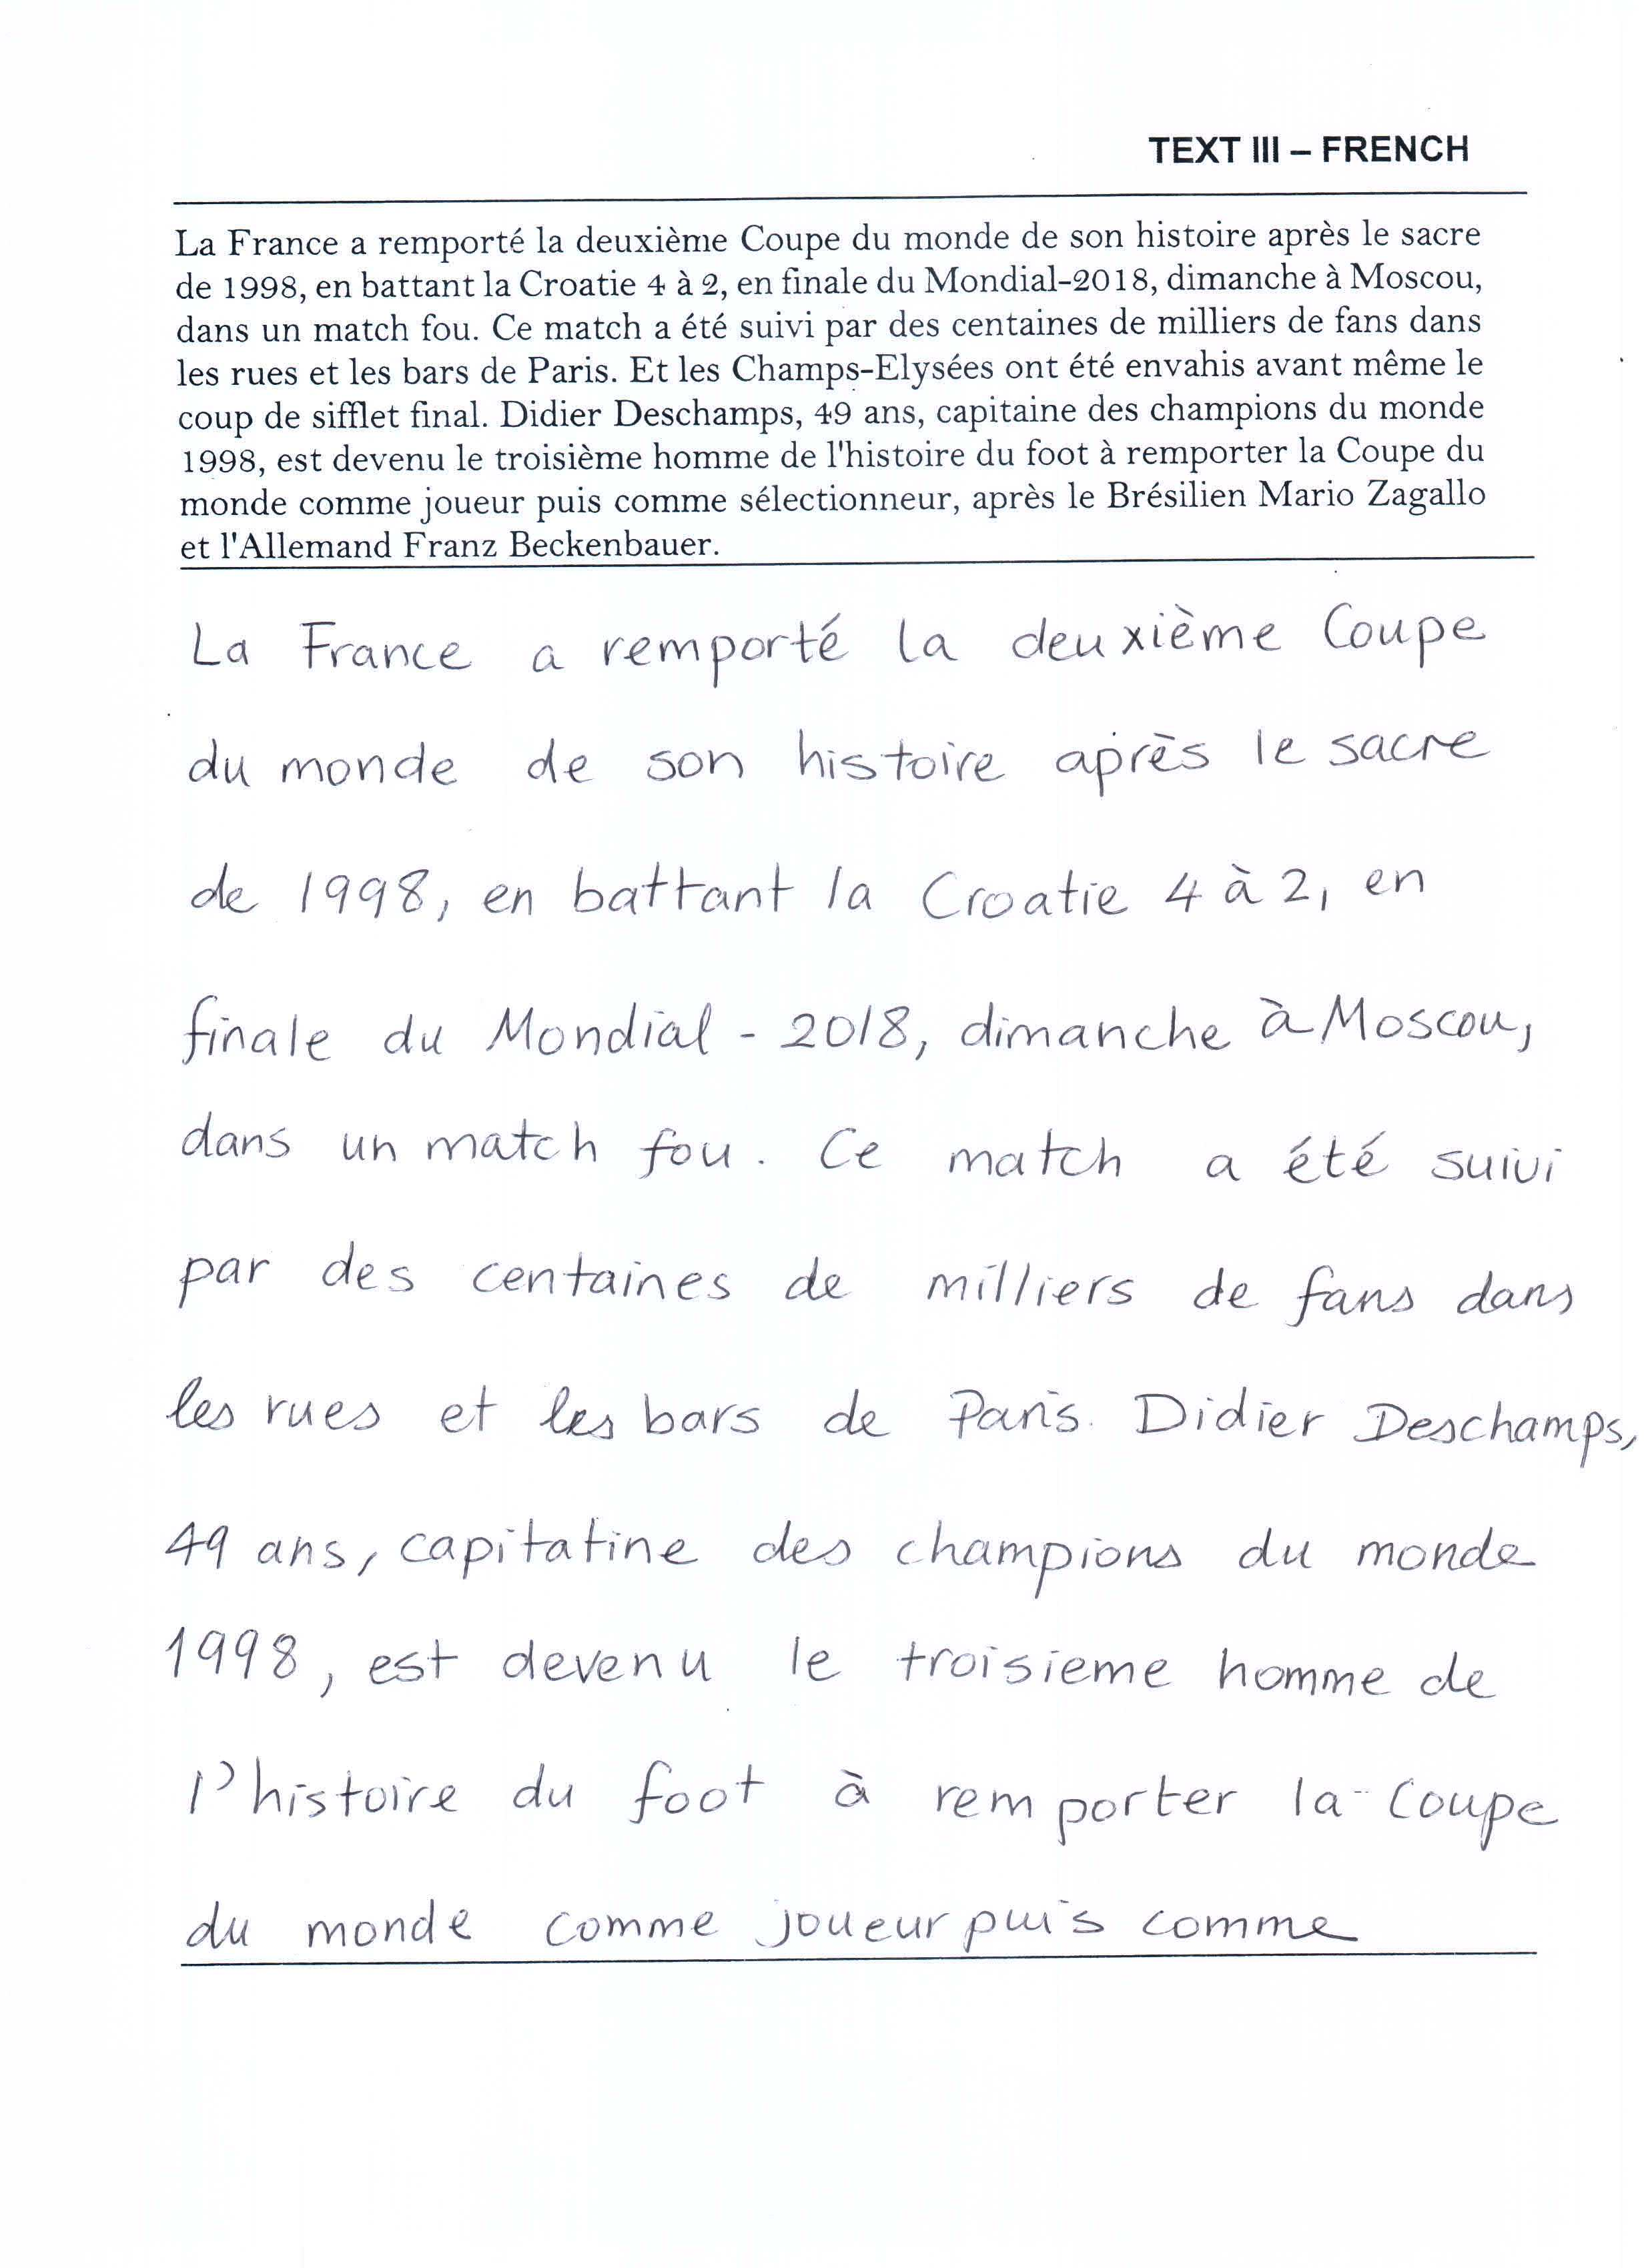
\includegraphics[width=0.4\textwidth]{images/5.jpeg}
    \caption{Image before clipping}
    \label{fig:clipping-example}
\end{figure}

\begin{figure}[h!]
    \centering
    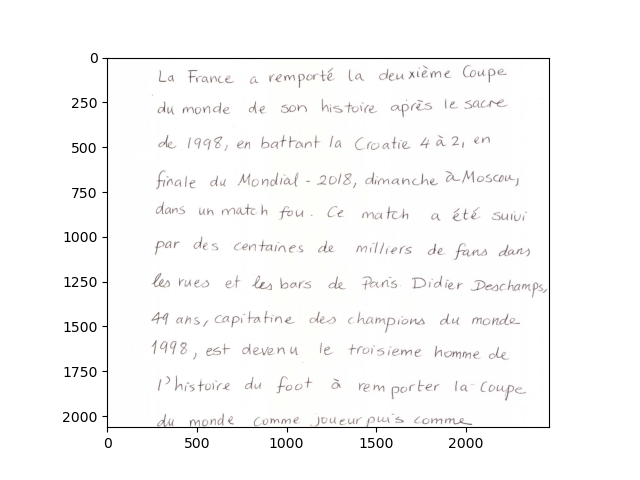
\includegraphics[width=0.4\textwidth]{images/img5_result.png}
    \caption{Image after clipping}
    \label{fig:clipping-result}
\end{figure}

\subsection{Line Segmentation}
As extracting features from lines is better than from the whole document, and classifying on each line helps to take a majority vote, We implemented a vectorized module to segment the document into lines using row histogram as shown in \ref{fig:histogram}. The docs are scanned vertically, so as shown in \ref{fig:bounding-boxes}, Detecting minima on a row histogram can get the boundaries to cut the lines on, as they are almost horizontal. We didn't use the concept of local minima in Detecting peaks as there is a lot of local minima that are not considered as line boundaries. We considered that the line boundary exists when there's an abrupt change in the histogram that makes it jump over $1/5$ of its mean. Some lines can be splitted into two lines, one of them has a small height. This happens because of different hand-writings. To tackle this problem, we filtered all lines that have black-pixel count less than $1/6$ of the mean of this count on all extracted lines. 

\begin{figure}[h!]
    \centering
    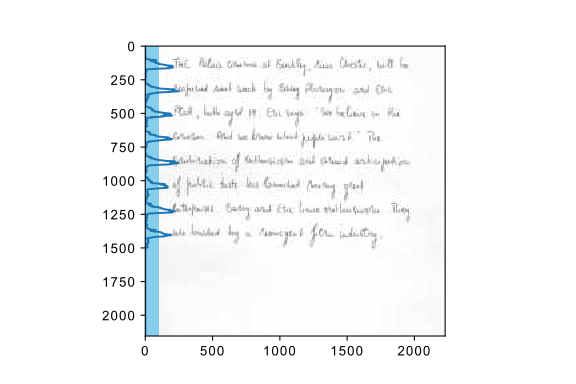
\includegraphics[width=0.5\textwidth]{images/histo.png}
    \caption{Row Histogram on Document to segment lines}
    \label{fig:histogram}
\end{figure}

\begin{figure}[h!]
    \centering
    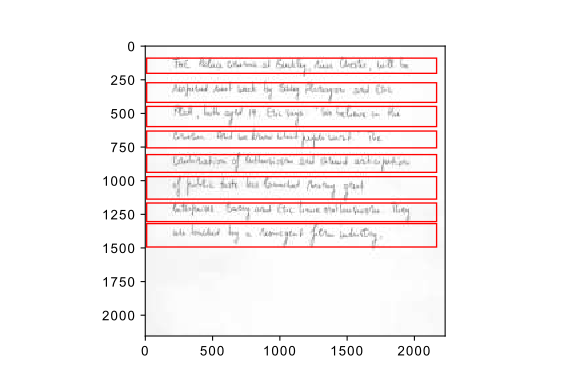
\includegraphics[width=0.5\textwidth]{images/BB.png}
    \caption{Resulting Bounding Boxes generated using Histogram}
    \label{fig:bounding-boxes}
\end{figure}

